\lab{Appendix}{More Matplotlib}{More Matplotlib}
\label{mpltables}

\objective{Display relevant matplotlib information}

The documentation for \li{matplotlib} can be frustrating to maneuver and relevant information is sometimes difficult to find. For this reason, we have supplied some of the more applicable and useful information here. 


\section*{Colours}
By default, every plot is assigned a different color specified by a ''color cycle". It can be overwritten by specifying what color is desired. \li{matplotlib} recognizes some basic built-in colours. 

\begin{tabular}
{|l||l|}
\hline
color & command \\
\hline
black & k \\
green & g \\
blue & b \\
red & r \\
cyan & c \\
magenta & m \\
yellow & y \\
white & w\\
\hline

\end{tabular}


The following displays how these colours can be  implemented. All the built-in colours are displayed for your convenience in Figure \ref{colours}
\lstinputlisting[style=fromfile]{colours.py}

\begin{figure} 
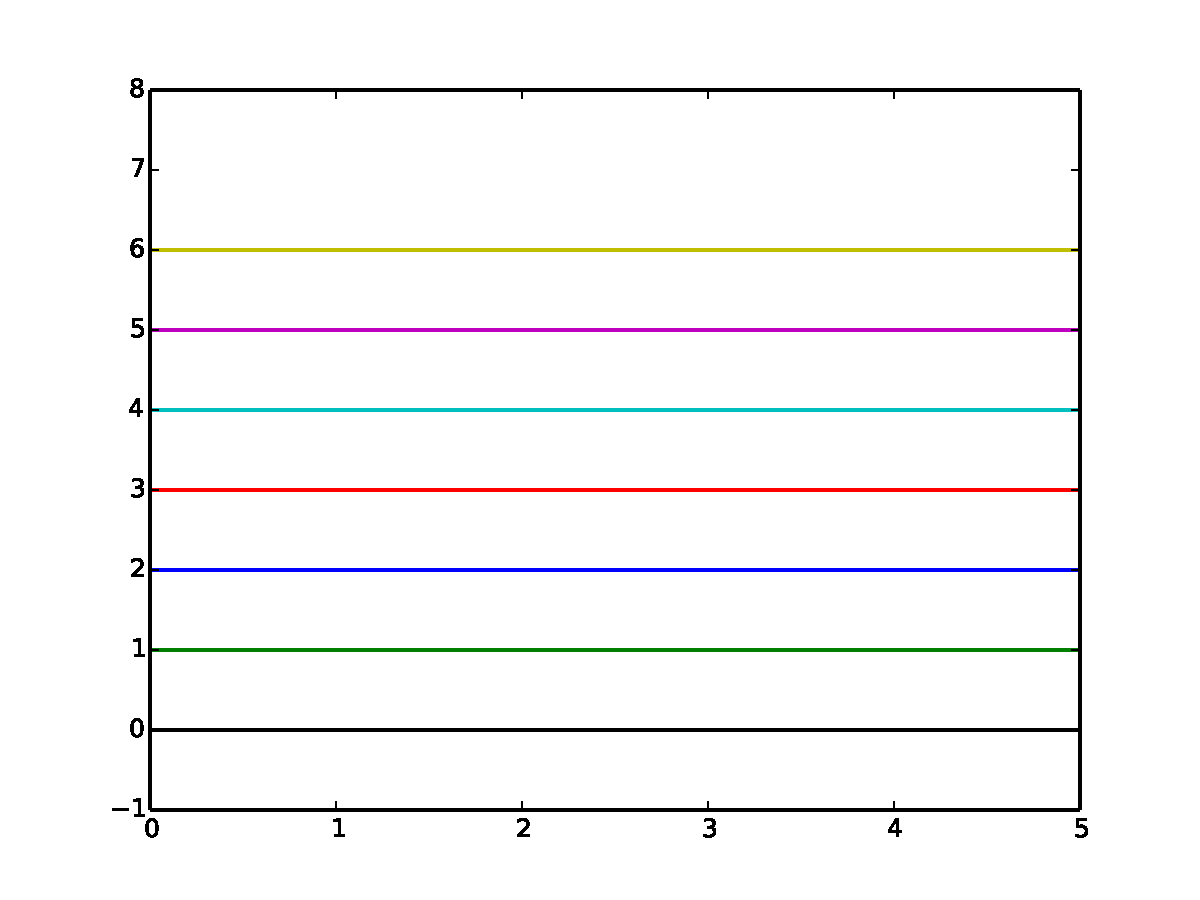
\includegraphics[width=\textwidth]{colours.pdf}
\caption{A display of all the built-in colours.}
\label{colours} 
\end{figure}


There are many other ways to specific colours. A popular method to access colours that are not built-in is to use a \li{RGB} tuple. Another way is to specify the color using an html hex string or its associated html color name like \li{DarkOliveGreen, FireBrick, LemonChiffon, MidnightBle, PapayaWhip,}, or \li{SeaGreen}. 

\section*{Axes}
You may have noticed the use of \li{plt.ylim([ymin, ymax])} in the previous code. This explicitly sets the boundary of the y-axis. Similarily, \li{plt.xlim([xmin, xmax])} can be used to set the boundary of the x-axis. 
Doing both commands simultaneously is possible with the \li{plt.axis([xmin, xmax, ymin, ymax])}. 
Remember that these commands must be executed after the plot. 

Another popular command is \li{plt.axis("tight")} which adjusts the axes so all data is visible and centered. 

\section*{lines}
\subsection*{width}
You may have noticed that the width of the lines above seemed thin considering we wanted to inspect the line colour. \li{linewidth} is a keyword argument that is defaulted to be \li{None} but can be given any real number to adjust the line width. 

The following displays how \li{linewidth} is implemented. It is displayed in Figure \ref{linewidth}
\lstinputlisting[style=fromfile]{linewidth.py}

\begin{figure} 
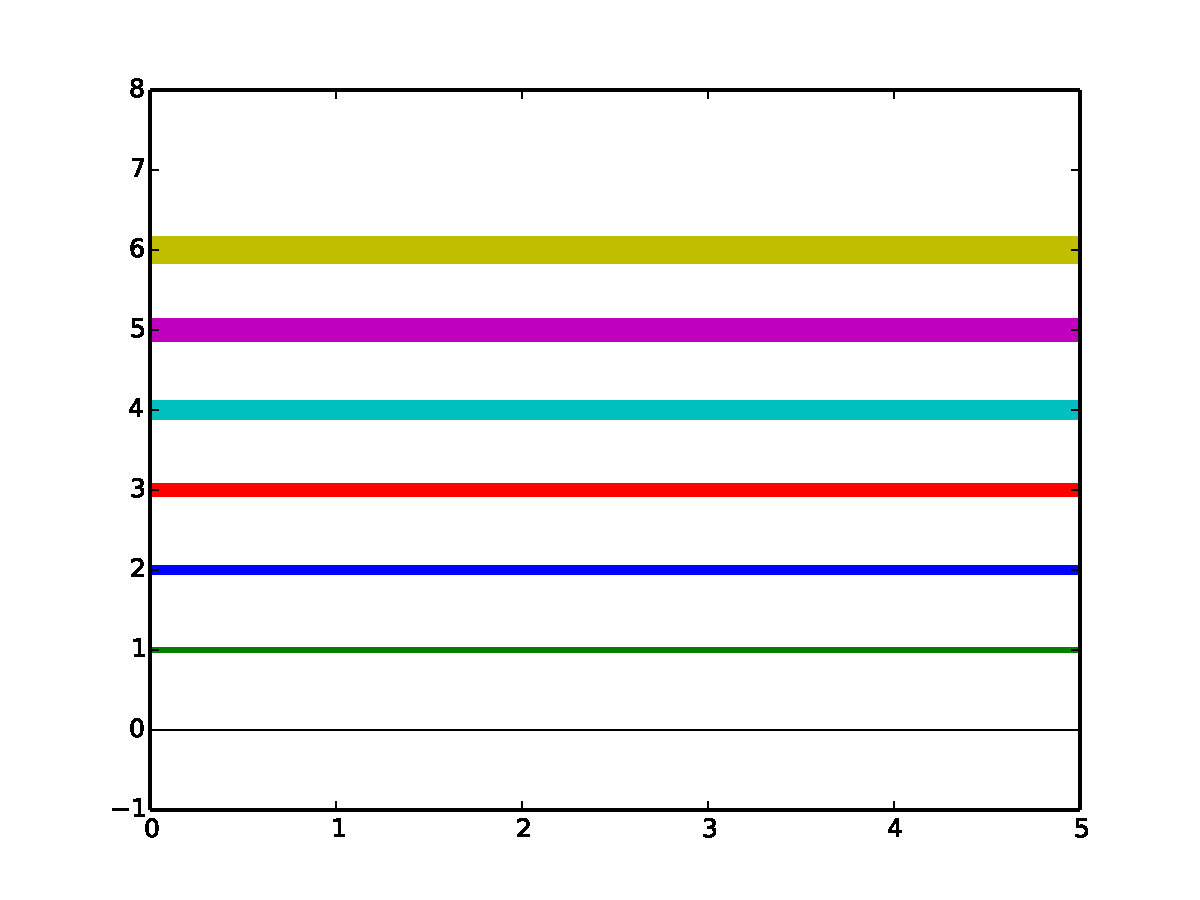
\includegraphics[width=\textwidth]{linewidth.pdf}
\caption{plot of varying linewidths.}
\label{linewidth} 
\end{figure}

\subsection*{style}
By default, plots are executed with a solid line style. We can easily change that. The following are accepted format string characters to indicate line style. 

\begin{tabular}
{|c||l|}
\hline
character & description \\
\hline
- & solid line style \\
-- & dashed line style\\
-. & dash-dot line style \\
: & dotted line style \\
. & point marker \\
, & pixel marker \\
o & circle marker \\
v & triangle\_down marker \\
\^{} & triangle\_up marker \\
$<$ & triangle\_left marker \\
$>$ & triangle\_right marker \\
1 & tri\_down marker \\
2 & tri\_up marker \\
3 & tri\_left marker \\
4 & tri\_right marker \\
s & square marker \\
p & pentagon marker \\
* & star marker \\
h & hexagon1 marker \\
H & hexagon2 marker \\
+ & plus marker \\
x & x marker \\
D & diamond marker \\
d & thin\_diamond marker \\
$|$ & vline marker \\
\_{} & hline marker \\
\hline 
\end{tabular}


The following displays how \li{linestyle} can be  implemented. 

It is displayed in Figure \ref{linestyle}
\lstinputlisting[style=fromfile]{linestyle.py}

\begin{figure} 
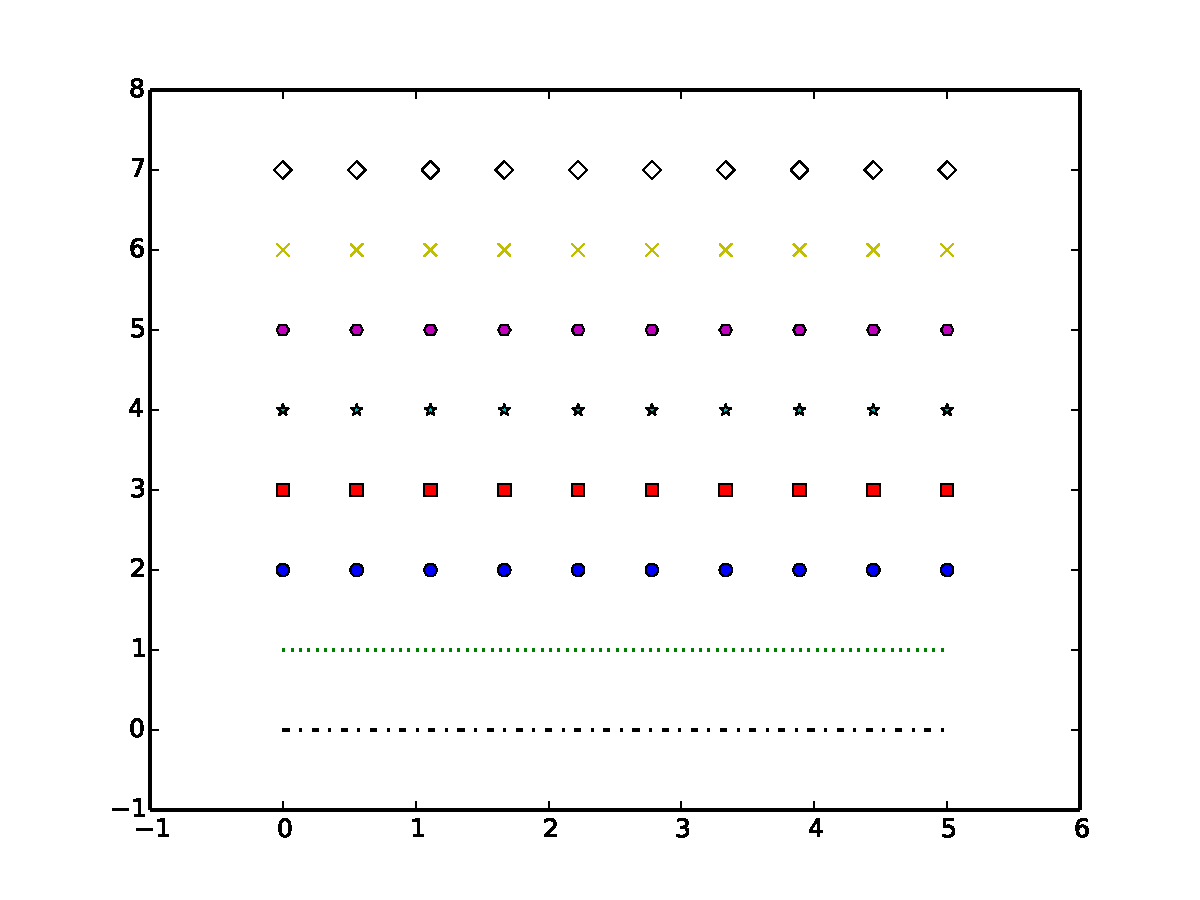
\includegraphics[width=\textwidth]{linestyle.pdf}
\caption{plot of varying linestyles.}
\label{linestyle} 
\end{figure}


\section*{Text}
It is also possible to add text to your plots. 

To label your axes, the \li{plt.xlabel()} and the \li{plt.ylabel()} can both be used. 

It is also possible to give your entire plot a title by using the \li{plt.title()} command. 

All of the \li{text()} commands can be customized with \li{fontsize} and \li{color} keyword arguments. 

We can add these elements to our previous example. 

It is displayed in Figure \ref{text}
\lstinputlisting[style=fromfile]{text.py}

\begin{figure} 
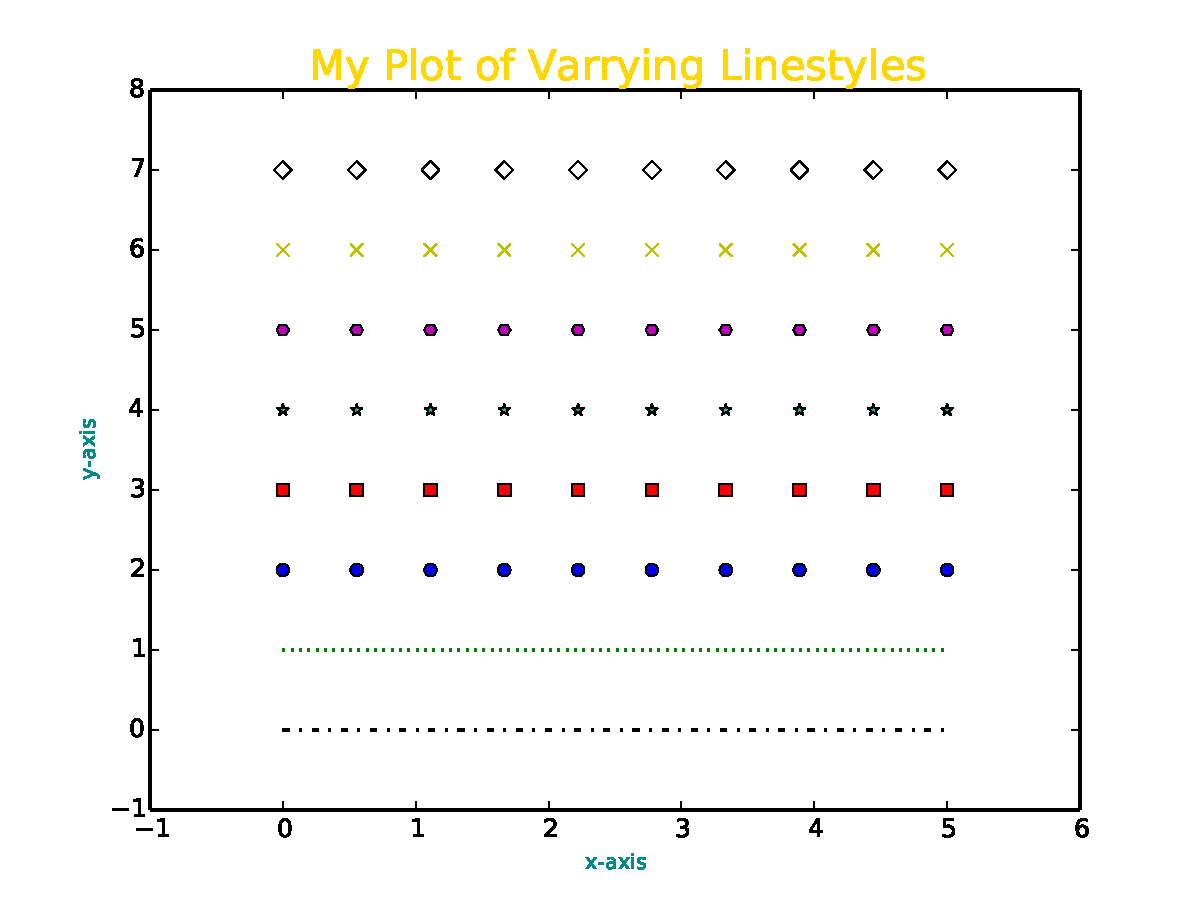
\includegraphics[width=\textwidth]{text.pdf}
\caption{plot of varying linestyles using text labels.}
\label{text} 
\end{figure}

